
\section{Background}

\textbf{Factor Graphs.}
Factor graphs are a pairwise formalism for expressing arbitrarily complex
relationships between random variables.
A factor graph $\mathcal{F}$, will contain a set of random variables, $r$
and a set of factors $f$. Random variables are connected to each other
through factors. Factors represent a mapping of the relationship to a 
real valued number.


\textbf{Markov Chain Monte Carlo Metropolis Hastings.}
Inference over complex factors graphs is computationally prohibitive.
Therefore, it is popular for researchers to use Markov Chain Monte Carlo (MCMC) 
approximation techniques to estimate probability values.
In particular, for large dense factor graphs MCMC Metropolis Hastings has
been shown to be a scalable and efficive technique for 
inference calculation~\cite{singh2011large}.

\ldots details of mcmc mh \ldots



\textbf{Cross-Document Coreference.}

Cross-Document coreference is resolving entities across document borders.
This problem is usually several orders of magnitude smaller when compared to within document entity resolution.
Solution to coreference comes in a variety of techniques.
We model entity resolution as a factor graph and use MCMC-MH for flexibility and the ability
to generalize the mathematically for other operations.

The distribution of entity sizes
In large text corpora, the sizes of entities follows the power law~\cite{singh12:wiki-links}.
For example, Figure~\ref{fig:entity-distribution} is a generated data set containing
40 million mentions and 3 million entities over 11 million web pages.

The mentions on disk can be represented as a large array of identifiers.
Entities are a collection of mentions and  can be represented as such.
In the worst case there is an equal number of entities and mentions.
This means each mention is its own individual entity.
In the other extreme, all the mentions may be a part of the same entity.


Doing pairwise comparison over clusters is $O(n^2)$.
For clusters larger than 1000 mentions calculating scores of the model
becomes extremely expensive.
Performing sophisticated techniques over smaller clusters could also 
add extra over head.

In this paper, we examine the trade-off of selecting techniques to
accelerate the feature computation process.


\begin{figure}
\centering
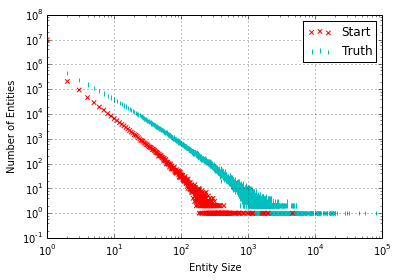
\includegraphics[width=\columnwidth]{media/start-vs-nd.png}
\caption{A distribution of entity sizes from the wiki-links corpus~\cite{singh12:wiki-links} with an initial start and the truth.}
\label{fig:entity-distribution}
\end{figure}





\section{Related Work}

In this paper use use sampling based ER over factor graphs.

Sameer Singh~\cite{singh2011large}
% Slides: http://people.cs.umass.edu/~sameer/files/largescale-acl11-ppt.pdf
% Slides: http://people.cs.umass.edu/~sameer/files/mcmcmc-emnlp12-ppt.pdf

Wick et al perform hierarchal compression of entities~\cite{Wick:2012:DHM:2390524.2390578}.


As we see, in Section~\ref{sec:microbenchmark} the entity sizes have a
large effect on the factor computation size.


